\documentclass[linenumbers, twocolumn]{aastex631}

\usepackage{graphicx}
\usepackage{amsmath}
\usepackage{amssymb}
\usepackage{newtxtext,newtxmath}
\usepackage{hyperref}
\usepackage{gensymb}

\newcommand{\vdag}{(v)^\dagger}
\newcommand\aastex{AAS\TeX}
\newcommand\latex{La\TeX}

\newcommand{\Msun}{\ensuremath{M_{\odot}}}
\newcommand{\Gyr}{\ensuremath{\textrm{Gyr}}}
\newcommand{\Myr}{\ensuremath{\textrm{Myr}}}
\newcommand{\yr}{\ensuremath{\textrm{yr}}}
\newcommand{\kpc}{\ensuremath{\textrm{kpc}}}
\newcommand{\pc}{\ensuremath{\textrm{pc}}}
\newcommand{\tocite}{\textcolor{blue}{cite}}
\newcommand{\FeH}{\ensuremath{[\textrm{Fe}/\textrm{H}]}}
\newcommand{\MgFe}{\ensuremath{[\textrm{Mg}/\textrm{Fe}]}}
\newcommand{\alphaFe}{\ensuremath{[\alpha/\textrm{Fe}]}}
\newcommand{\tform}{\ensuremath{t_{\textrm{form}}}}
\newcommand{\dex}{\ensuremath{\textrm{dex}}}

\newcommand{\red}[1]{\textcolor{red}{#1}}

%% Reintroduced the \received and \accepted commands from AASTeX v5.2
% \received{March 1, 2021}
% \revised{April 1, 2021}
%\accepted{\today}

\shorttitle{The Milky Way's Phoenix Phase}
\shortauthors{Beane et al.}

\graphicspath{{./}{fig/}}

\begin{document}

\title{Rising from the Ashes: How the Milky Way Got Its Scars}

\author{Angus Beane}
\affiliation{Center for Astrophysics $|$ Harvard \& Smithsonian, Cambridge, MA, USA}

\author{Lars Hernquist}
\affiliation{Center for Astrophysics $|$ Harvard \& Smithsonian, Cambridge, MA, USA}

\author{et al}

%% Mark off the abstract in the ``abstract'' environment. 
\begin{abstract}
  The nuclear abundance distribution of stars encodes the history of the gas-phase abundance in the Milky Way. Without a large, unbiased sample of stellar ages, the exact timing and nature of this history must be \textit{inferred} from the abundances. In the two-dimensional plane of \alphaFe-\FeH, it is now clear that two separate populations exist - the low-$\alpha$ and high-$\alpha$ sequences. A restatement of this fact is that the distribution of \alphaFe{} is bimodal at a fixed Fe. Structure in the nuclear abundance distribution can arise from many processes - proposals include radial migration, high-redshift clump formation, and various effects associated with galaxy mergers, among others. In this work, we demonstrate another possible avenue for structure formation with clear observational predictions. We propose that the Galaxy underwent a starburst followed by a brief (hundreds of Myr) quiescent phase. A natural consequence of this quiescent phase is that stars in the valley of the bimodality do not form because: (1) the absence of enrichment from high-mass stars leads to a rapid reduction in \alphaFe{}, and (2) any time the gas spends in the abundance valley is deemphasized in the present day distribution because the star formation rate is lower. With a set of idealized merger simulations, we demonstrate the feasibility of this proposal. The starburst and quiescent phase can result from a merger, but it is not a necessary component of the theory. This ``phoenix hypothesis'' predicts a gap in stellar ages at a fixed \FeH{} and that stars which form directly after this gap would have lower \alphaFe{} than stars which form slightly later.
\end{abstract}

%% Keywords should appear after the \end{abstract} command. 
%% The AAS Journals now uses Unified Astronomy Thesaurus concepts:
%% https://astrothesaurus.org
%% You will be asked to selected these concepts during the submission process
%% but this old "keyword" functionality is maintained in case authors want
%% to include these concepts in their preprints.
\keywords{Classical Novae (251) --- Ultraviolet astronomy(1736) --- History of 
astronomy(1868) --- Interdisciplinary astronomy(804)}

\section{Introduction} \label{sec:intro}
Elements heavier than hydrogen are produced through nuclear fusion. After Big Bang Nucleosynthesis, this only occurs in compact objects. The distribution of elemental abundances in the gas-phase of a galaxy is determined by a complicated combination of physical processes - stellar evolution and supernovae, gas accretion, galaxy mergers, gas outflows from stellar and AGN feedback, metal mixing and diffusion, etc.

By necessity, stars inherit the constituitive properties of the gas cloud from which they formed. Moreover, the surface abundance of stars do not change over time.\footnote{For the most part.} We therefore have the unique opportunity to examine the historical record of the gas-phase abundance of a galaxy by way of the distribution of the surface abundances of stars. Because the processes which give rise to this distribution are complex, there is almost certainly some structure in this distribution for every galaxy. However, it has only been definitively measured in the Milky Way.

The distribution of elemental abundances is a high dimensional space (\red{e.g. up to 8 billion elements by XYZ}). However, this space is highly degenerate, and so the effective number of dimensions is much smaller - even possibly compressed to just \FeH and age \citep{2019ApJ...883..177N}.

Two elements in particular have received particular interest - iron and $\alpha$-elements (elements produced through the $\alpha$-process, typically tracked with just Mg). Type Ia and Type II supernovae are the main contributors of elemental enrichment. Iron is broadly produced in both types, and so its abundance is a proxy for the total metallicity of a star. $\alpha$-elements, on the other hand, are mainly produced in Type II supernovae. The ratio of $\alpha$-elements to iron is then a measure of the relative contributions of Type Ia and II to the enrichment of a parcel of gas. It has therefore become common to compress the high-dimensional abundance space to the two dimensional \FeH-\alphaFe plane.

In this plane, it is now well-established that a significant bimodality exists in the Milky Way \red{cite a boatload}.





Elemental enrichment is accounted for in modern galaxy formation models, though the validity of the yield tables is suspect. It is not known if the yields (i.e., the amount of metals produced by the SN) used in such models are accurate. This issue is further compounded by the fact that the mixing of metals is unresolved and is sensitive to numerical choices (e.g., Eulerian codes being generally more diffusive than Lagrangian). To make matters even worse, the inflows and outflows of gas from galaxies is sensitive to the choices of the feedback model, which has a strong impact on a galaxy's elemental history.




The last\footnote{i.e., not ongoing} significant merger was between the
proto-Milky Way disk and the {\em Gaia}-Sausage-Enceladus (GSE)
(\textcolor{red}{spell check}) satellite galaxy. The stellar debris from this
merger constitutes $\sim50\%$ \textcolor{red}{check} of the inner ($r<?\,\kpc$)
stellar halo. It may have also led to a tilted, triaxial dark matter halo
(\textcolor{red}{cite}).

The GSE merger is often invoked (\textcolor{red}{cite}) to explain the observed
bimodality in the \textcolor{red}{alpha iron} abundance plane
(\textcolor{red}{cite}). Because GSE-mass galaxies are expected to have a lower
star formation efficiency than proto-Milky Way-mass galaxies
(\textcolor{red}{cite}), the gas from GSE should be relatively metal poor. The
gas from GSE thus dilutes the gas in the proto-Milky Way, ``resetting'' the
chemical abundance of the Milky Way.

However, it has also been claimed that the \textcolor{red}{alpha iron}
bimodality can be explained through secular processes. \textcolor{red}{Sentence
explaining the basic concept.} The argument is not that the GSE merger did not
happen, but rather that it is not {\it necessary} and might not even be {\it
sufficient} to explain the bimodality. Ongoing work to detect the bimodality in
external galaxies may shed further light on the topic (\textcolor{red}{cite}).

Investigating GSE-like mergers in cosmological simulations is a rich and active
area of research. Many mergers believed to be similar to the GSE merger have
been identified in the literature (\textcolor{red}{cite}). \textcolor{red}{Blah
blah argue blah blah. And also blah blah argues blah blah.}

While much has been learned from GSE-like mergers in cosmological simulations,
they are not conducive to controlled experiments. It is possible to change the
mass of satellites through genetic modification (\textcolor{red}{Pontzen}), and
the GSE analog can be removed entirely (\textcolor{red}{Cooke cite}). However,
to our knowledge, no method has been applied to change the orbital parameters of
such a merger. It is also somehwat unclear if the circumgalactic media of
proto-Milky Way mass galaxies at $z\sim2$ are properly simulated.

In this work, we present hydrodynamic simulations of a controlled merger between
a GSE analog and the $z\sim2$ proto-Milky Way. 

\begin{figure*}
  \centering
  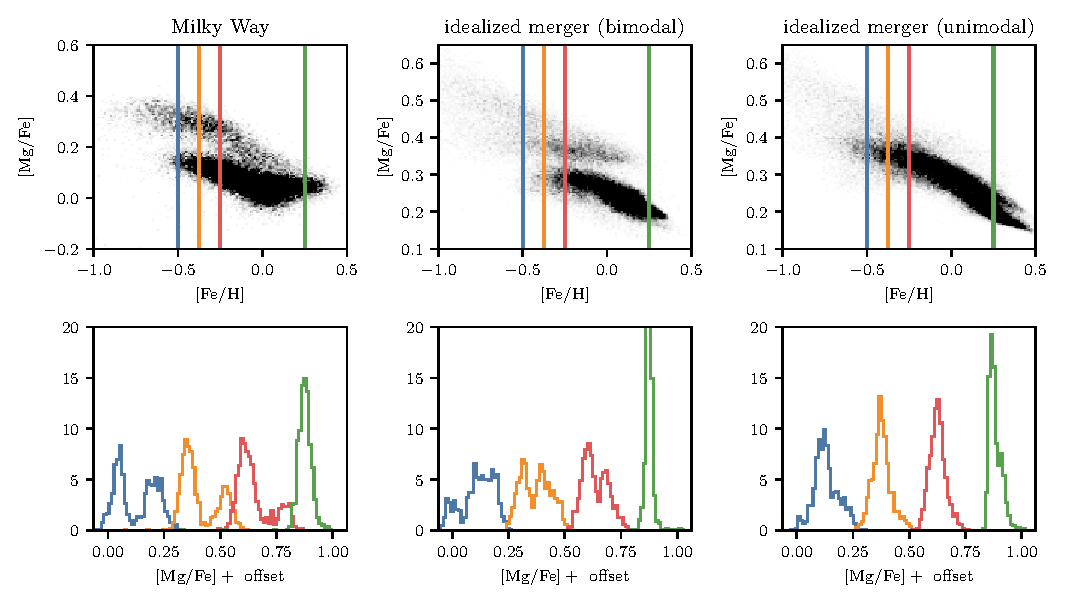
\includegraphics[width=\textwidth]{figure1.pdf}
  \caption{\textbf{The abundance bimodality seen in the Milky Way can be reproduced in some idealized merger simulations.} In the upper panels, we show the distribution of stars in the \MgFe-\FeH plane. The left panel shows the observed distribution in the Milky Way from ASPCAP \red{cite}, while the right two panels show two idealized merger simulations. The idealized merger simulations are nearly identical, except that the bimodal simulation has a starting radius of $129\,\kpc$, while the unimodal simulation has a starting radius of $142\,\kpc$. We emphasize that the labels ``unimodal'' and ``bimodal'' are of the \textit{outcome} of the simulation, and do not reflect a particular choice in the setup. The bottom panels show the distribution of \MgFe at fixed \FeH. The colors indicate the fixed \FeH values, which are $-0.5$, $-0.375$, $-0.25$, and $0.25$. The Milky Way (left panels) exhibits a strong bimodal distribution of \MgFe at various \FeH. The idealized merger simulation marked as bimodal (center panels) also exhibits a bimodal distribution of \MgFe, though the structure is not as strongly defined. The idealized merger simulation marked as unimodal exhibits only weak structure, if any at all.}
  \label{fig:fig1}
\end{figure*}

\section{Methods}\label{sec:methods}

\subsection{Gaseous Halos}\label{ssec:gashalo} 

The nature of the circumgalactic media of local galaxies remains largely
uncertain. It is unclear whether the constraints we have on the local universe
apply to the circumgalactic media of $z\sim2$ galaxies. Nonetheless, we persist.

We assume the CGM of the Milky Way and GSE can be modelled using a $\beta$ profile,
\begin{equation}
  \rho(r) = \rho_0 \left( 1 + \left(\frac{r}{r_c}\right)^2 \right)^{-\frac{3}{2}\beta}\textrm{.}
\end{equation}
However, a $\beta$-profile has been shown to be a reasonable fit to the density
profile of galaxy clusters and of the $L_{*}$ galaxy NGC 3221. Whether or not
such a profile extends to lower mass galaxies at $z~2$ is unclear, but to our
knowledge there is no better motivation for another profile.

Our construction of the Milky Way and GSE CGM follows
\citet{2023MNRAS.tmp.2070B}. In particular, we set $\beta=2/3$ and $r_c=0.22
r_s$, where $r_s$ is the scale length of the dark matter halo. For the Milky Way
and GSE, $r_c=9$, $6.5\,\textrm{kpc}$, respectively. For the present study we
keep $\beta$ and $r_c$ fixed and instead vary the central density $\rho_0$. Our
fiducial values are $9.61\times10^{-5}$ and $7.57\times10^{-5}\,\Msun/\pc^3$ for
the Milky Way and GSE, respectively.

A useful metric for assessing the central density is by the universal baryon
fraction $f_{\textrm{B}}$ -- i.e., the ratio between the mass in baryons to the
mass in dark matter within $R_{200}$ as compared to the mean ratio of the
universe.\footnote{To be explicit,
$f_{\textrm{B}}=(M_{\textrm{b}}/M_{\textrm{c}})/(\Omega_{\textrm{b}}/\Omega_{\textrm{c}})$,
where $M_{\textrm{b}}$ and $M_{\textrm{c}}$ are the mass of baryons and cold
dark matter within $R_{200}$, and $\Omega_{\textrm{b}}$ and
$\Omega_{\textrm{c}}$ are the mean baryon and cold dark matter densities of the
universe.} For our fiducial central densities, this value is $1.07$ and $0.28$
for the Milky Way and GSE respectively using the universal values from
\cite{2014AA...571A..16P}. An early argument by 

\begin{figure*}
  \centering
  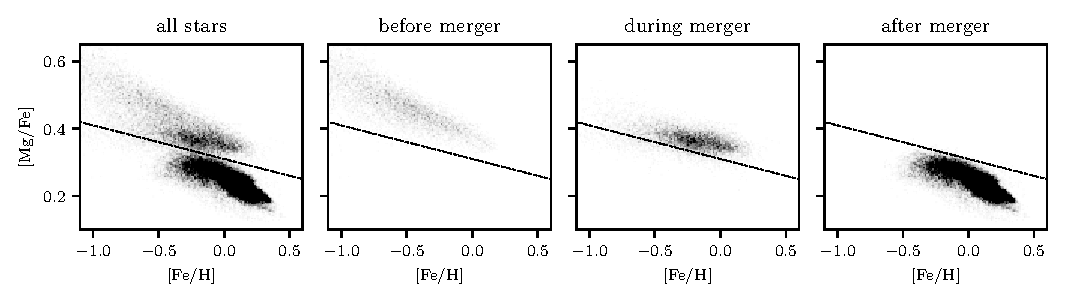
\includegraphics[width=\textwidth]{before_after.pdf}
  \caption{\textbf{The high-$\alpha$ sequence forms before the merger, the low-$\alpha$ sequence forms after the merger.} This plot shows the sequence of events leading to the build-up of the low- and high-$\alpha$ sequences for our fiducial bimodal simulation. We have separated the high- and low-$\alpha$ sequences by a dashed line at $-0.1\FeH + 0.31$, which was chosen by eye to lie in the trough. The left panel shows all star particles in our solar neighborhood cut. The middle left panel shows the star particles that form before the merger ($\tform < 1.5\,\Gyr$), which form a weak sequence of star particles at the lowest \FeH and highest \MgFe. The middle right panel shows the star particles that form during the merger ($1.5\,\Gyr < \tform < 2.5\,\Gyr$). These star particless form the portion of the high-$\alpha$ sequence closest to the trough, and the density of star particless is higher than those that form before. The middle right panel shows the star particles which form after the merger ($\tform > 2.5\,\Gyr$). These star particles form almost entirely below the trough.}
  \label{fig:before_after}
\end{figure*}

\begin{figure}
  \centering
  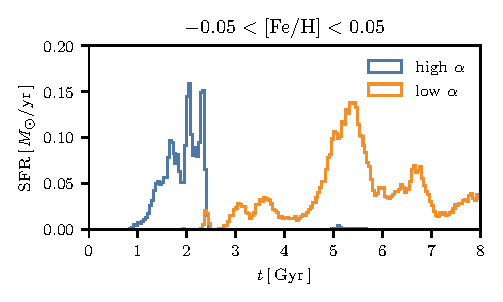
\includegraphics[width=\columnwidth]{before_after_sfh.pdf}
  \caption{\textbf{At fixed metallicity, the low- and high-$\alpha$ sequence are cleanly separated in time, with an intervening quiescent period.} Here we show the star formation history of the high- and low-$\alpha$ sequences. The blue (low-$\alpha$) and orange (high-$\alpha$) histograms correspond to the dashed line cut made in the \MgFe-\FeH plane in Figure~\ref{fig:before_after}, at a fixed metallicity of $\FeH\sim0$. One can see that there is a nearly perfect separation in time between the formation of the high-$\alpha$ and low-$\alpha$ sequence, except for a brief overlap which can be attributed to the inadequacy of the linear cut model of the two sequences. Separating the formation periods lies a quiescent period with a duration of $\sim300\,\Myr$. \red{make sfr per dex}.}
  \label{fig:before_after_sfh}
\end{figure}

\begin{figure}
  \centering
  \includegraphics[width=\columnwidth]{before_after_sfh_by_iron.pdf}
  \caption{\textbf{The timing of the quiescent period which divides the high- and low-$\alpha$ sequences is metallicity dependent.} The star formation history of stars at various fixed metallicities ($\FeH\sim0$, $-0.25$, and $-0.5\,\textrm{dex}$). As in Figure~\ref{fig:before_after_sfh}, there is a quiescent period period which separates the formation of the low- and high-$\alpha$ sequence \red{maybe a better way to show this?}. However, one can see that the timing of the quiescent period is metallicity-dependent. It occurs earlier at lower metallicity, by $\sim300\,\Myr$ for the metallicities shown in this plot. \red{make sfr per dex}.}
  \label{fig:before_after_sfh_by_iron}
\end{figure}

\begin{figure*}
  \centering
  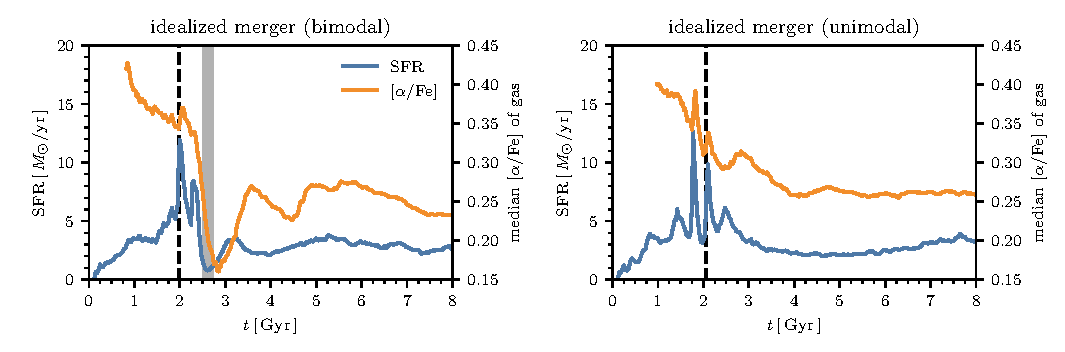
\includegraphics[width=\textwidth]{SFR_alpha.pdf}
  \caption{\textbf{A global suppression of star formation is associcated with a decrease in \MgFe{}, which is seen in the bimodal simulation but not in the unimodal simulation.} Here, we show both the SFR of the central galaxy ($r<15\,\kpc$) and the median \MgFe{} for gas at $2\,\kpc<r<5\,\kpc$ at a fixed \FeH{} bin centered on $-0.2$ with width $0.02\,\dex$. The left panel shows the bimodal simulation while the right panel shows the unimodal simulation. The time of the merger (i.e., the second pericenter) is indicated by the vertical dashed line. In the bimodal simulation, the star formation is suppressed after the merger. This suppression of star formation is associated with a sudden drop in the median \MgFe{} of the gas. Neither the suppression of star formation nor the drop in \MgFe{} are seen in the unimodal simulation.}
  \label{fig:SFR_alpha}
\end{figure*}


\bibliography{ref}{}
\bibliographystyle{aasjournal}

%% This command is needed to show the entire author+affiliation list when
%% the collaboration and author truncation commands are used.  It has to
%% go at the end of the manuscript.
%\allauthors

%% Include this line if you are using the \added, \replaced, \deleted
%% commands to see a summary list of all changes at the end of the article.
%\listofchanges

\appendix

\section{Modelling the Milky Way and GSE at $z=2$}


Our merger simulations are built upon reasonable models of both the Milky Way
and GSE at $z\sim2$. Much is uncertain about the properties of the Milky Way and
GSE at these redshifts.  We describe the motivation for the choices made in
constructing these models.

\subsection{The Milky Way}
We adopt a \citet{1990ApJ...356..359H} profile for our dark matter halo. For its
structural parameters, we follow \citet{2021ApJ...923...92N} and set its mass
and scale length to be $5\times10^{11}\,\Msun$ and $40.4\,\kpc$, respectively.
This matches a \citet{1996ApJ...462..563N} profile with
$R_{200}=129\,\textrm{kpc}$ and concentration $c_{200}=3.8$
(\textcolor{red}{check this}).

Milky Way-progenitor galaxies have been observed up to $z=?$ with well-formed
disks, and more massive galaxies have dynamically cold disks up to $z\sim6$. We
therefore assume the thick disk is settled and in place at $z=2$. We use the
structural parameters of the thick disk from . It is presently unclear if before
the GSE merger the Milky Way disk was already thickened, or if it was thickened
by the merger. Some simulations indicate that only prograde mergers efficiently
thicken disks (\textcolor{red}{check and cite}). For this work, we assume the
disk is already thick.

For the bulge, we assume the present day classical bulge was already in place at
$z=2$. Measurements of the structural parameters of the classical bulge are
uncertain due to contamination by the boxy peanut bulge generated by the bar
(\textcolor{red}{cite}). Some even argue that the classical bulge does not exist
(\textcolor{red}{cite}). Nonetheless, we assume the bulge properties from
\textcolor{red}{Bland Hawthorn, but check}. Specifically, we assume a Hernquist
bulge with $M_{\textrm{bulge}}=?$ and $a=?$.

We assume a gas disk with an exponential surface density profile and scale
length matched to the stellar disk. The vertical profile is set by the condition
of gravito-hydrostatic equilibrium as described in (\textcolor{red}{Springel}).
Varying the gas fraction of the disk strongly influences the SFR of the galaxy.
We therefore varied the gas fraction of the disk until we reached a target
SFR.\footnote{Note that when we varied the gas fraction of the disk, we kept the
mass (and scale length) of the stellar disk constant. Therefore, the total mass
of the disk changes as we vary the gas fraction.} \textcolor{red}{People} argue
that in order for the thick disk to have formed thick, the SFR of the disk at
$z\sim2$ needed to be $\sim15\,\Msun/\yr$. It is not necessary for the disk to
be thick at $z\sim2$, so we acknowledge this is an upper limit on the SFR. We
adopt an initial gas fraction of $0.7$ which results in an average SFR of
$\sim16\,\Msun/\yr$.

Finally, we note that the present day Milk Way has a well-formed bar. It is
expected to have formed within a few Gyr of the GSE merger, so it is unclear if
the bar formed before, as a result of, or after the merger. This is not a focus
of the current work. The presence of a classical bulge and the disk being
dynamically hot is sufficient for the disk to be stable against bar
instabilities.

\section{Cause of Suppressed Star Formation}

\begin{figure*}
  \centering
  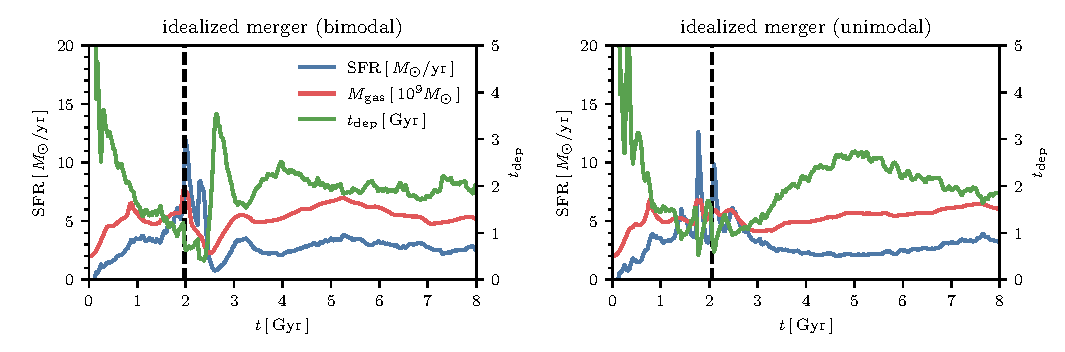
\includegraphics[width=\textwidth]{SFR_Mgas_tdep.pdf}
  \caption{\textbf{The suppression of star formation in the bimodal simulation is associated with both a reduction in gas mass as well as an increase in the depletion time.} The drop in star formation (blue line) at $\sim2.5-3\,\Gyr$ is associated with both a reduction in the total gas mass (red line) as well as an increase in the depletion time (green line). This shows that the SFR suppression is a result of both less gas mass and more inefficient star formation. \red{Should this only include the bimodal? Also, move to appendix?}}
  \label{fig:SFR_Mgas_tdep}
\end{figure*}

\begin{figure}
  \centering
  \includegraphics[width=242.26653pt]{MdotBH_rsep.pdf}
  \caption{\textbf{The bimodal merger is associated with high accretion rates onto the central SMBH.} Around the time of each pericentric passage, and slightly after, the accretion rate (blue line) becomes very high. Here, it is shown as a fraction of the Eddington accretion rate. During the merger, the accretion rate reaches as high as Eddington at some times, but is always above $10\%$. The orbital separation between the central and satellite is shown in the orange line.}
  \label{fig:MdotBH_rsep}
\end{figure}

\end{document}

% End of file `sample631.tex'.

% Ness 2019 
